\documentclass[tikz,
  margin=3pt,
  convert,
  convert={
    outext=.png,
    command=\unexpanded{
      pdftocairo -r 300 -png \infile % 将生成的pdf文件转换为png图像
    }
  }
  ]{standalone}
  
\usepackage{pgfplots}
\pgfplotsset{compat=newest}

\begin{document}

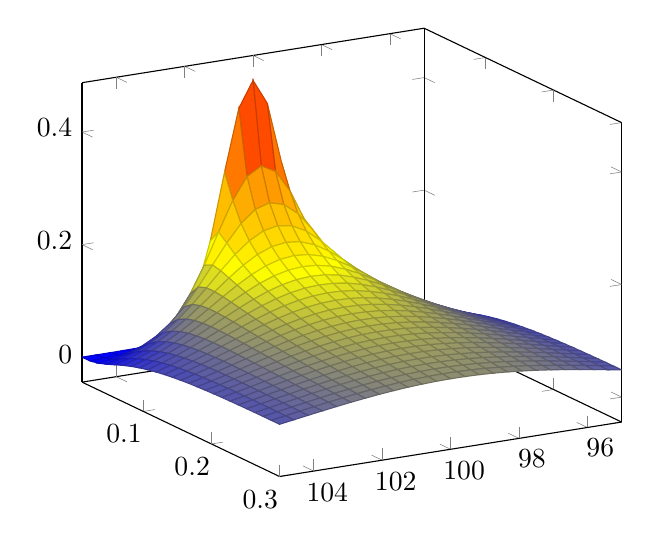
\begin{tikzpicture}[
  declare function={
    Nprime(\x)                 = 1/(sqrt(2*pi))*exp(-0.5*(pow(\x,2))); 
    d2(\x,\y,\KK,\RR,\SIG)     = (ln(\x/\KK)+(\RR-(pow(\SIG,2)/2)*\y))/(\SIG*(sqrt(\y)));
    myfun(\x,\y,\KK,\RR,\SIG)  = exp(-\RR*\y)*Nprime(d2(\x,\y,\KK,\RR,\SIG))/(\x*\SIG*sqrt(\y));
  },
  ]
  \begin{axis}[
    y domain=0.01:0.3,
    domain=95:105,
    view={150}{20}
    ]
    \addplot3[surf] {myfun(x,y,100,0,0.09)};
  \end{axis}
\end{tikzpicture}

\end{document}

%%% Local Variables:
%%% mode: latex
%%% TeX-master: t
%%% End:
